\chapter{Approaches}\label{chapter:approaches}
In this chapter, the various approaches taken on getting insights using classical statistical, \ac{ML} and Data Mining techniques are explained. The actual outcomes of the \ac{ML} models and Data Mining algorithms are outlined in chapter \ref{chapter:findings}.

\section{Data exploration}
Before training \ac{ML} models it is important to understand what type of underlying data one is working with. The section \ref{chapter:preprocessing} on preprocessing explains the individual features and explains why the split of the data based on feature \textit{op} has been done. These findings originate from exploring the data in the first place, and understand which preprocessing steps are to be done to gain insights that are meaningful. One intuitive way to understand the relations between the features is by exploring the correlation between them. 

\subsection{Correlation}\label{correlationchapter}
A correlation, as the name suggests, describes the relationship between two features. In this thesis, the Pearson product-moment correlation coefficient is covered as defined by Salkind \parencite{salkind2011statistics}. This correlation coefficient measures the relationship between two values, giving a value in the range $[-1,1]$. Positive values for features X and Y indicate a relationship, where if the value of a feature X increases, the feature Y increases too. Negative values indicate the that the decrease of feature X results in an increase of feature Y. \\
The coefficient r between two features X and Y is calculated using the formula \ref{correlationformula}.

\begin{equation} \label{correlationformula}
r = \frac{n\sum_{i=1}^{n} (x_i - \bar{x})(y_i - \bar{y})}{\sqrt{n\sum_{i=1}^{n} (x_i - \bar{x})^2 \cdot n\sum_{i=1}^{n} (y_i - \bar{y})^2}}
\end{equation}
where:
\begin{align*}
r & \text{ is the Pearson correlation coefficient}, \\
n & \text{ is the number of data points}, \\
x_i \text{ and } y_i & \text{ are individual data points of X and Y}, \\
\bar{x} & \text{ is the mean of X}, \\
\bar{y} & \text{ is the mean of Y}.
\end{align*}
\\\\
This correlation can be calculated comparing all features, resulting in the correlation matrix as described by Papoulis et al. \parencite{papoulis2002probability}. It is symmetric along the diagonal, as the Person correlation is symmetric in nature as well. The figure \ref{fig:cormatrix} describes the correlation in the dataset collected in this thesis. Non-numeric features have been excluded for better viewability. It can be observed that the lower right section of the matrix displays high absolute values. This can be easily explained, since these features are output features, which are highly correlated between each other, including the target feature \textit{time}. 
\begin{figure}[h]
  \centering
  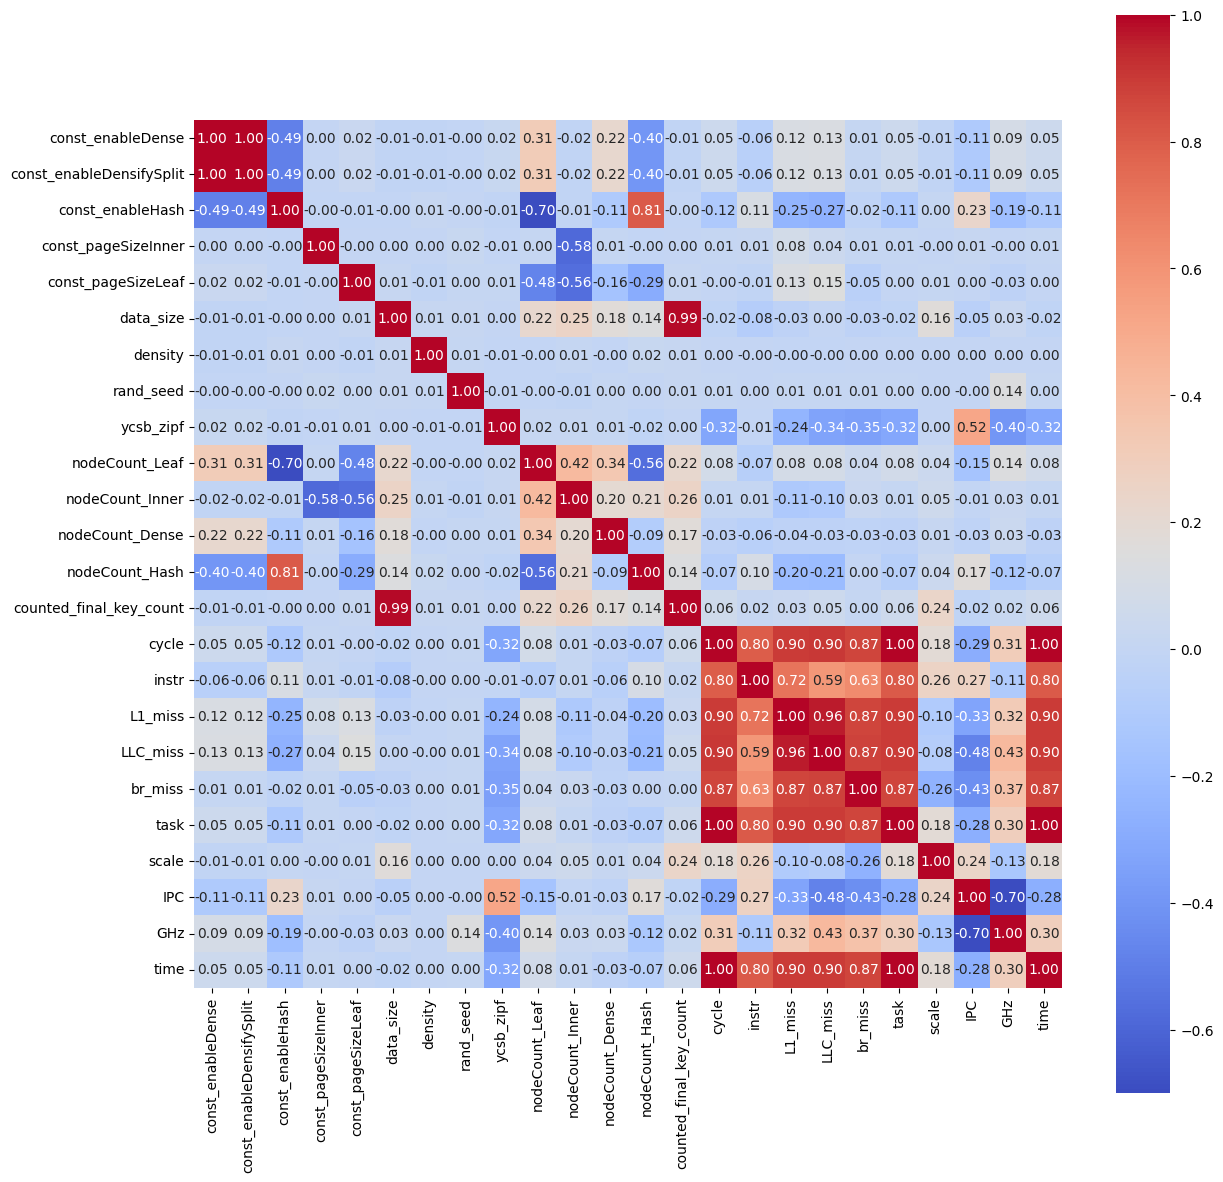
\includegraphics[width=0.8\textwidth]{images/correlation_matrix.png}
  \caption{Correlation matrix of the full dataset}
  \label{fig:cormatrix}
\end{figure} 
\\\\
Figure \ref{fig:cortime} represents the correlation coefficients between the feature \textit{time} and all other features. Some features are omitted from this figure, due to their constant values resulting in undefined behavior. The figure further highlights the high correlation between the output features and time, by displaying the output features in red and input features in blue. This highlights the importance of excluding these features as inputs to the \ac{ML} models. Including these features, would make it much easier for the \ac{ML} models to calculate the feature \textit{time} with high precision. However, such a scenario would be an inaccurate representation, since the output features are not available for new values and the goal of this thesis is to find correlation between input features and the feature \textit{time}.  
\\\\
Additionally, it can be observed that looking at the input features and their statistical correlation to feature \textit{time}, does not give promising insights, which is why \ac{ML} models are used to learn more complex relationships between the input and the feature \textit{time}. 
\begin{figure}[H]
  \centering
  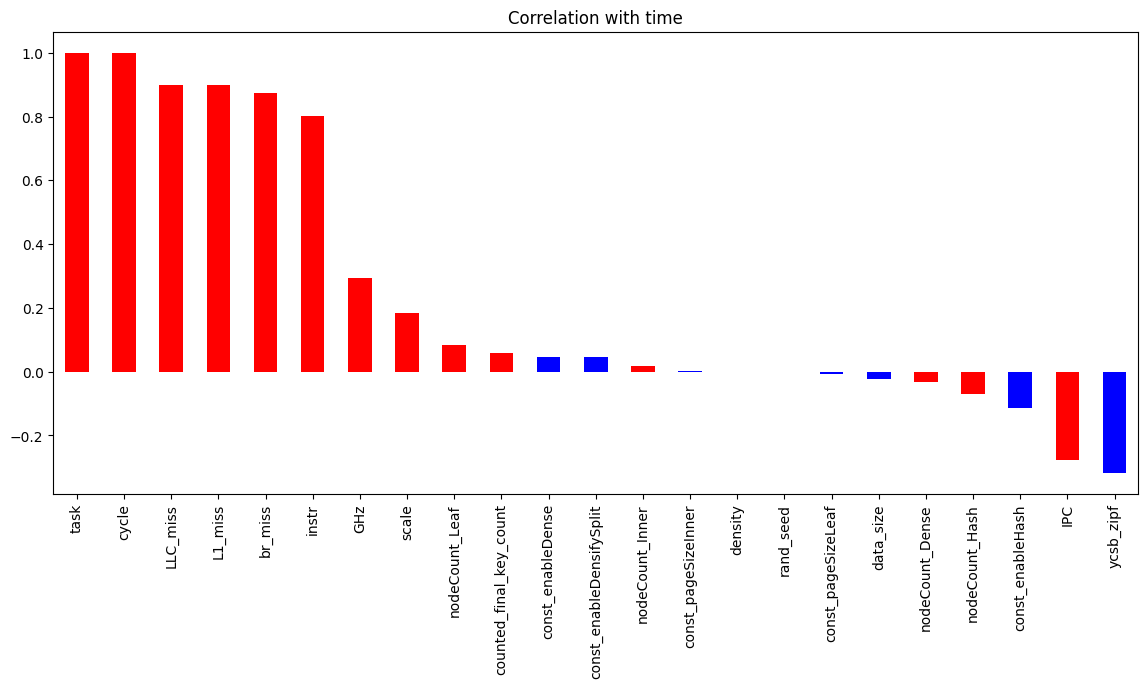
\includegraphics[width=0.8\textwidth]{images/correlation_with_time.png}
  \caption{Correlation of features with feature \textit{time}}
  \label{fig:cortime}
\end{figure}

\section{Classification models}
This section describes which classification models are used and what they do in a general sense. Before the individual \ac{ML} models are used, however, one needs to define, what is classified and what the metrics are used to distinguish good from bad models. In this thesis, the classification problem is defined as follows:
\\\\
Since the feature \textit{time} is a continuous value, it is not reasonable to classify each possible value as one class. Therefore, the values are split into 10 sections, based on the values. The class 1 indicates that the value is in the lowest 10\% of the data, meaning that it is among the fastest values. The class is stored as the feature \textit{percentile bracket}. For this, the following code is used to create the feature:

\begin{lstlisting}[language=Python]
df['percentile bracket'] = pd.qcut(df['time'], q=10, labels=False,
                                duplicates='drop') + 1
\end{lstlisting}
To make sure that the \ac{ML} model can be evaluated, a metric needs to be used on data, which the model has not been fed beforehand. Therefore, the data is split into a train- and a test set. This thesis uses an 80:20\% train/test split, which according to Joseph \parencite{joseph2022optimal} is a common ratio. In the paper \parencite{joseph2022optimal}, Joseph suggests using a ratio depending on the number of parameters, however, since this thesis aims to get insights into the data and not the best performing model, the simpler, static ratio split is applied.\\\\
Using the test set, a metric can calculate the usefulness of the model. The metric being used in this thesis is the accuracy score, as defined by \textit{scikit-learn} in \parencite{sklearnm19:online}. This score calculates the fraction of the correctly classified samples from the test set.
\\\\
Since the data has been split between the four values of feature \textit{op}, there are four models trained and therefore four metrics are compared per model type. 


\subsection{Decision Tree}
The Decision Tree classification, according to Zhou's definition in “Machine Learning” \parencite{zhou2021machine}, is a \ac{ML} model, which classifies data by creating a set of rules in a tree structure. The rules can be thought of if-then rules. At the leaf of the tree, the class of the value is defined. The Decision Tree can be built using a recursive algorithm, which continuously splits the set of data points in a node based on defined splitting rules until one of the termination conditions is met. In the book “Machine Learning” \parencite{zhou2021machine} Zhou defines the following three conditions on a node:
\begin{itemize}
  \item All data points are of the same class. 
  \item All data points have the same feature values, or there is no more feature to split. 
  \item There is no data point in the node.
\end{itemize}
The implementation that is used in this thesis \parencite{sklearnt33:online} allows further terminating conditions, such as the maximum depth of the tree, the maximum number of leaf nodes or a minimum number of data points required for a split of a node. 
\\\\
In the book “Machine Learning” \parencite{zhou2021machine}, Zhou further outlines that in order to determine the split, a higher \textit{purity} of the new child nodes is attempted to be achieved. The \textit{purity} is commonly measured by the \textit{information gain}, given in formula \ref{infogainformula}. Calculating the \textit{information gain} requires the \textit{entropy} of data, which is given in formula \ref{entropyformula}.  
\begin{equation} \label{entropyformula}
 \text{Ent}(D) = -\sum_{k=1}^{|y|} p_k \log_{2} p_k 
\end{equation}
where: 
\begin{align*}
\text{Ent}(D) & \text{ is the entropy of the data set}, \\
|y| & \text{ is the number of classes}, \\
p_k & \text{ is the proportion of the } k \text{th class}
\end{align*}
It is assumed that the classes are labelled $k=1,2,...,|y|$.
\begin{equation} \label{infogainformula}
\text{Gain}(D, a) = \text{Ent}(D) - \sum_{v \in \text{Values}(a)} \frac{|D_v|}{|D|} \text{Ent}(D_v)
\end{equation}
where:
\begin{align*}
\text{Ent}(D) & \text{ is the entropy of the dataset } D \\
\text{Values}(a) & \text{ is the feature} \\
|D_v| & \text{ is the number of instances for which feature } a \text{ has value } v \\
\text{Ent}(D_v) & \text{ is the entropy of the dataset } D_v
\end{align*}
The library \textit{scikit-learn} \parencite{sklearnt33:online} by default uses the splitting criterion \textit{Gini impurity} instead of \textit{entropy}. The \textit{Gini impurity}, according to Zhou \parencite{zhou2021machine} is defined in formula \ref{giniimpurityformula}.
\begin{equation} \label{giniimpurityformula}
\text{Gini}(D) = 1- \sum_{k=1}^{|y|} p_k^2
\end{equation}
where:
\begin{align*}
\text{Gini}(D) & \text{ is the Gini impurity of the dataset } D \\
|y| & \text{ is the number of classes} \\
p_k & \text{ is the proportion of the } k \text{th class}
\end{align*}
During experimentation of this thesis, practically, the results between using the criterion \textit{entropy} and \textit{Gini impurity} yielding minimal differences below a $0.5\%$ accuracy. Since no criterion yielded consistently better results, for the context of this thesis the criterion \textit{Gini impurity} is chosen. 
\\\\
Zhou \parencite{zhou2021machine} states that these formulae assume discrete values, which is why for continuous values a simple discretization technique is used, where the middle index of the sorted values is taken. This middle index is then used for splitting the feature values into two intervals, which can be taken as discrete values to calculate the splitting criterion.

\subsection{Random Forest}
The Random Forest classifier by \textit{scikit-learn} \parencite{sklearne64:online} takes the idea of a Decision Tree classifier and trains multiple Decision Trees with varied configurations. According to Zhou \parencite{zhou2021machine}, the variations vary the available features at each step. Additionally, the available data points are varied, with repeating data points across variations. 
\\\\
Zhou \parencite{zhou2021machine} further explains, that this method is part of the idea of Ensemble learning, where multiple models are trained and each value is then evaluated on all models and later the results are combined to give a final result. After training a given number of Decision Trees, the class is determined by giving one vote to each model. This method provides the benefit of better controlling over-fitting the models, since each time only a subset of data points from the training set is used. 

\subsection{Gradient Boosting}
According to Masui \parencite{AllYouNe72:online}, Gradient Boosting is an ensemble technique, which is built on the idea of training a "weak" decision tree and iteratively improving on it, by taking the loss function into account and using gradient descent. The loss function used in this thesis is the \textit{log\_loss}, which is the idea used in Logistic Regression \ref{LogisticRegression} and according to \textit{scikit-learn} \parencite{sklearne30:online} is a good idea for classification with probabilistic outputs. The figure \ref{fig:gradientboost} visualizes the flow of a Gradient Boosting model. The weights assigned to each "weak" decision tree is based on the loss function. The mechanism of how gradient descent is used in each iteration during training is out of the scope of this thesis.

\begin{figure}[H]
      \centering
      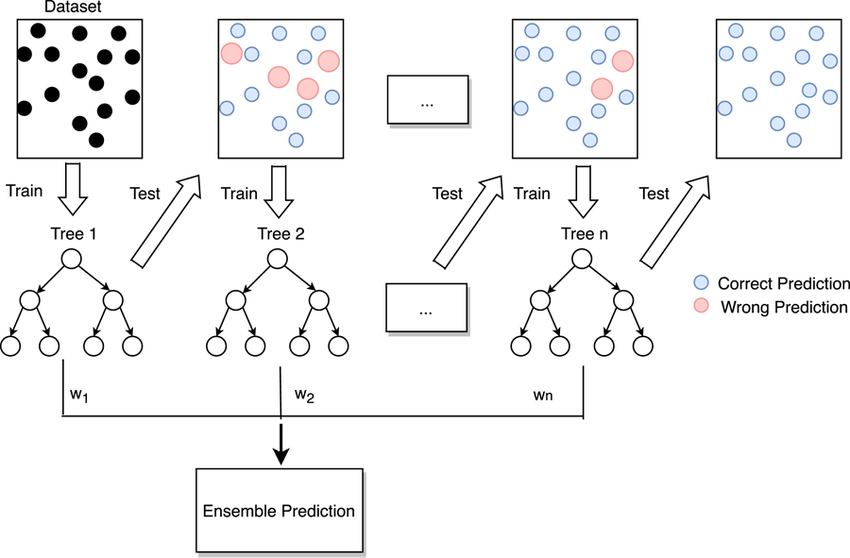
\includegraphics[width=0.5\textwidth]{images/gradientBoosting.png}
      \caption{Gradient Boosting flow diagram \parencite{gradientBoosting} }
      \label{fig:gradientboost}
  \end{figure}

\subsection{Neural network}
In the book \parencite{zhou2021machine} Zhou describes that there exist a number of types of neural networks, like Radial Basis Function networks, Adaptive Resonance Theory networks or Self-Organizing Map networks. However, the one described and used in this thesis is the Multilayer Perceptron (MLP) Classifier as defined by \textit{scikit-learn} \parencite{117Neura38:online}. According to Bishop \parencite{bishopML} the MLP is considered the most successful model, as it is of practical value for statistical pattern recognition. The MLP is also known as a feed-forward neural network. An example for an MLP is visualized in figure \ref{fig:mlp_sample}. The layer on the left is known as the input layer, where each node, also known as a neuron, represents one feature. The rightmost layer, the output layer, contains the output features, which in this example case is a scalar value, which in the case of MLP Classifiers would be the class of the value. The middle layer represents the hidden layer. There can be multiple hidden layers defined, each with a different amount of neurons. Additionally, each layer contains a \textit{bias}, typically referred to as the $0$th weight, $w_0$, in the layer. 
\begin{figure}[h]
      \centering
      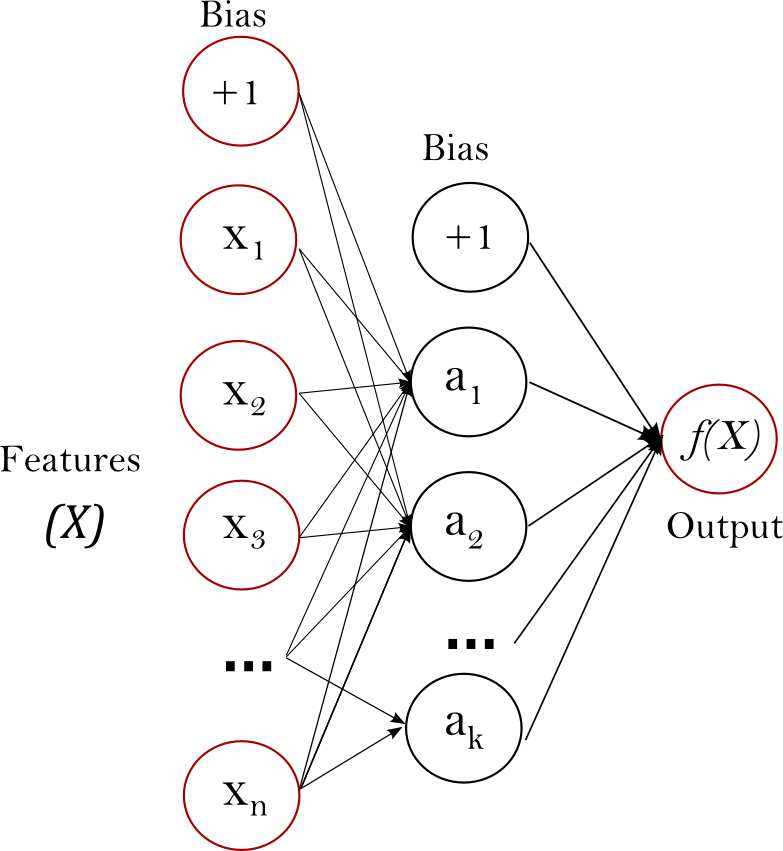
\includegraphics[width=0.5\textwidth]{images/mlp_example.png}
      \caption{MLP with one hidden layer \parencite{117Neura38:online} }
      \label{fig:mlp_sample}
  \end{figure}
As stated by Bishop \parencite{bishopML} and \textit{scikit-learn} \parencite{117Neura38:online}, each neuron, take the values from the previous layers and calculate a weighted sum $w_0 + w_1x_1 + w_2x_2 + ... + w_mx_m$, which consequently is put into a typically nonlinear activation function. Choosing the activation function can be done based on domain knowledge about the underlying data and its distribution.
\\\\
During experimentation of this thesis, the following activation functions yielded results with the highest accuracy. The \textit{ReLu} (Rectified Linear Unit) function $f(x)=max(0,x)$ and the \textit{Identity} function $f(x)=x$. In the end, \textit{ReLu} resulted in a slightly higher accuracy, therefore the results of this activation function are presented in the chapter on findings \ref{chapter:findings}.
\\\\
The neural network training process can be defined as follows:
\begin{enumerate}
    \item \textbf{Initialization}: The weights and biases are assigned random values.
    \item \textbf{Forward Pass}: At each layer the data from the previous layer is weighted summed, transformed and passed forward to the consequent layer.
    \item \textbf{Loss Calculation}: A loss function compares the calculated output for a validation set, which is not used in forward pass, with the actual output. 
    \item \textbf{Backpropagation}: The loss is then propagated backwards through the network by calculating gradients using mathematical techniques like the chain rule in calculus. 
    \item \textbf{Gradient Descent}: The gradients calculated in backpropagation are used to adapt the parameters in the loss-minimizing direction. Multiple Gradient Descent algorithms can be used, including \textit{Adam}, defined in \parencite{kingma2017adam}, and \textit{Stochastic Gradient Descent}. 
    \item \textbf{Iterations}: Steps 2 - 5 are iterated, gradually improving the network's performance. The training is terminated once the loss stops to decrease or starts to increase. Other terminating conditions can be set to the maximum number of iterations, time limit or by integrating other performance metrics. 
\end{enumerate}
This thesis does not delve into the detailed mathematical principles underlying backpropagation and gradient descent techniques. However, one characteristic of MLP Classifiers is that it is sensitive to feature scaling, which is why \textit{scikit-learn} \parencite{117Neura38:online} suggests using the \textit{StandardScalar}, as defined in \parencite{sklearnp90:online}, which transforms the data in such a way that each feature has a mean of zero and a standard deviation of one. This indeed improved the performance of some models trained in this thesis. In one case, this improvement increased the accuracy from around $4\%$ to more than $80\%$. The precise results are outlined and discussed in chapter \ref{chapter:findings}.

\subsection{Logistic regression} \label{LogisticRegression}
Despite what the name suggests, logistic regression actually is a classification model. The base case for logistic regression considers a binary classification, meaning that only two classes are considered, true and false. The logistic function, otherwise known as logistic sigmoid or sigmoid function, is used to identify the probability of an input belonging to a class. The logistic function is outlined in the formula \ref{logitfunc}. 
\begin{equation}\label{logitfunc}
    g(z) = \frac{1}{1 + e^{-z}}
\end{equation}
The figure \ref{fig:logitReg} visualizes the binary case of a logistic regression with one feature on the x-axis. The threshold value is set to 0.5 implying that results of the logistic function above 0.5 are classified as the class 1. 
\begin{figure}[h]
      \centering
      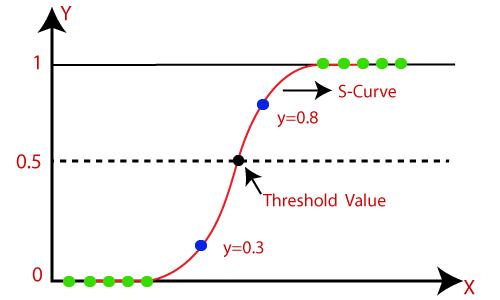
\includegraphics[width=0.5\textwidth]{images/logisticReg.png}
      \caption{Logistic regression example \parencite{Logistic19:online} }
      \label{fig:logitReg}
  \end{figure}
\\\\
The idea of binary classification case, can be extended to support multiple classes. The implementation used in this thesis extends the case by using \textit{multinomial logistic regression} with \textit{cross-validation}. This thesis does not go into the details of the multinomial logistic regression model, however the main idea can be summarized as follows.\\
To predict the class of a value the model takes a weighted sum of the input features for each possible class, puts the output into the softmax function, as defined in \ref{softmax}. These results are then put into the logistic function, which are then interpreted as the probability for each class. The most likely class is chosen to classify the value. \\ 

\begin{equation}\label{softmax}
    \text{softmax}(z_i) = \frac{e^{z_i}}{\sum_{j=1}^{K} e^{z_j}}
\end{equation}
\\
Following the suggestion of \parencite{CrossVal0:online}, to prevent overfitting and performing poorly on unseen data the cross-validation \textit{scikit-learn} implementation \parencite{sklearnl39:online} is used in this thesis. The concept is visualized in figure \ref{fig:crossval}. The training set is taken and split into $k$ disjoint subset. Afterward, each time a different subset is omitted from the training set and used as the testing set for that iteration. Following this, the results are averaged to create an evaluation result. This thesis set the parameter $k$ to 10, as it is, according to Zhou \parencite{zhou2021machine}, the most commonly used value.

\begin{figure}[h]
      \centering
      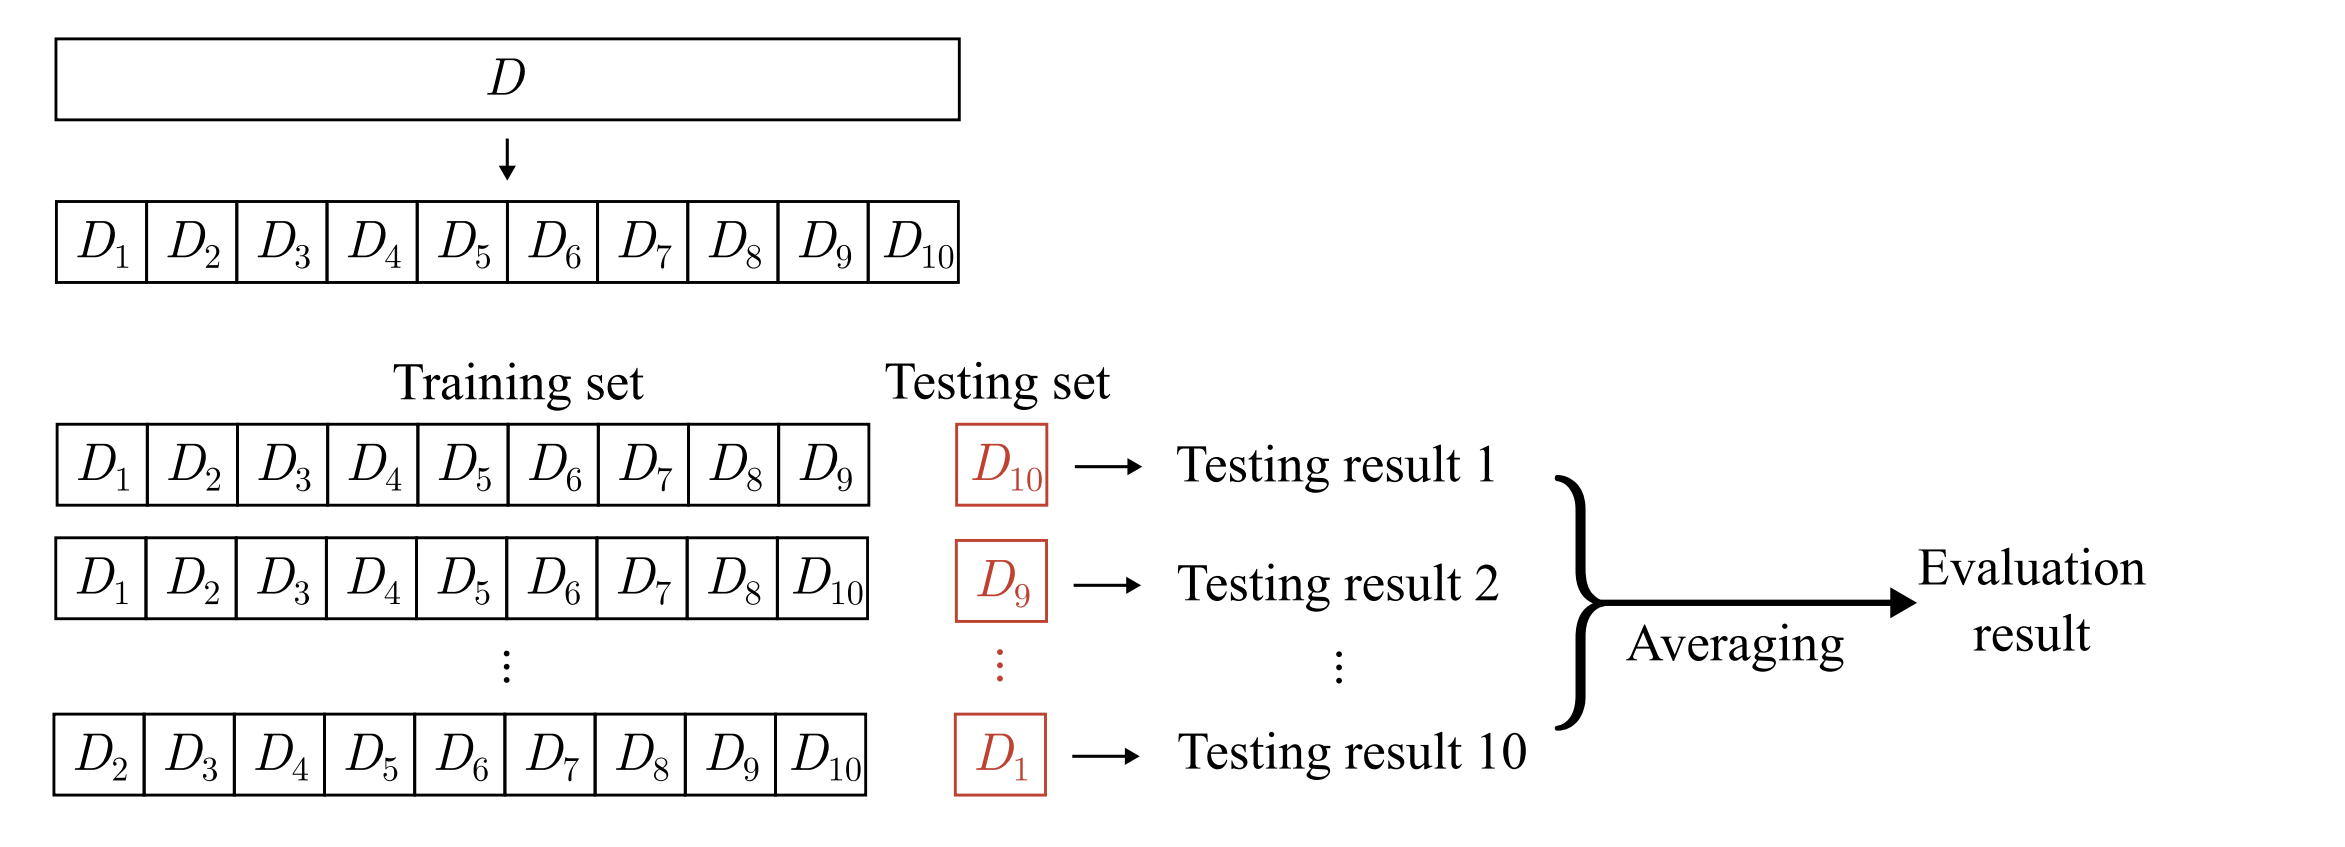
\includegraphics[width=0.5\textwidth]{images/crossvalidation.png}
      \caption{Cross validation example \parencite{zhou2021machine} }
      \label{fig:crossval}
  \end{figure}

\section{Regression models}
This section describes which \ac{ML} regression models have been used and gives an overview of how the individual models work. Since regression models are able to target a continuous feature, the target feature is the feature \textit{time}, without the need for more preprocessing.\\\\
To evaluate the performance of the models, the same procedure as with classification models with an 80/20 train/test split of data is employed. In contrast to the classification models, this thesis uses two metrics to evaluate the individual models.
\\\\
\textbf{RMSE} stands for Root Mean Squared Error, which, as the name suggests, is the root of the \textbf{MSE} metric. The MSE metric itself is the most commonly used metric, according to Zhou \parencite{zhou2021machine}, and it takes the mean of the squared errors, as defined in \ref{mseformula}. 
\begin{equation}\label{mseformula}
MSE = \frac{1}{n} \sum_{i=1}^{n} (y_i - \hat{y}_i)^2
\end{equation}
Despite the fact that RMSE is a metric in the same units as the target variable, this thesis uses the metric MSE. This is due to the already minuscule scale of the feature \textit{time}. 
\\\\
Additionally, since very small numbers are expected as errors, it is a good idea to make sure that the models actually perform better than the simplest model possible, which would be taking the average of the entire dataset. The \textbf{$R^2$}, as described by \textit{scikit-learn} in \parencite{sklearnm99:online}, also known as the coefficient of determination, typically yields results between 1, the perfect predictions, and 0, the average of the dataset. It can, however, also yield negative values, when the models perform more poorly than the average-case. The \textbf{$R^2$} is defined in formula \ref{rsquaredformula}
\begin{equation}\label{rsquaredformula}
R^2 = 1 - \frac{\sum_{i=1}^{n} (y_i - \hat{y}_i)^2}{\sum_{i=1}^{n} (y_i - \bar{y})^2}
\end{equation}
where:
\begin{align*}
R^2 & \text{ is the coefficient of determination} \\
n &  \text{ is the number of data points} \\
y_i & \text{ is the actual value of the } i^{th} \text{ record} \\
\hat{y}_i & \text{ is the predicted value of the } i^{th} \text{ record} \\
\bar{y} & \text{ is the mean of actual values of all records}
\end{align*}

\subsection{Linear regression}
According to Bishop \parencite{bishopML} the simplest linear model, and also the one used in this thesis, is the linear regression model. The model attempts to create a linear combination of input variable to create an output value. The model itself can be defined as in formula \ref{linregformula}. 
\begin{equation}\label{linregformula}
y = w_0 + w_1 x_1 + w_2 x_2 + \ldots + w_n x_n
\end{equation}
where:
\begin{align*}
y & \text{ is the target feature} \\
x_1, x_2, \ldots, x_n & \text{ are the features} \\
w_0, w_1, \ldots, w_n & \text{ are the weights representing the slopes of the regression line} 
\end{align*}
As Alto describes in \parencite{Understa37:online}, to estimate the weights of the Ordinary Least Squares (OLS) method is used, which minimizes the sum of squared differences. The details of this method include  differentiating the sum of squared differences with respect to each coefficient, setting the derivatives to zero, and solving the equation. 
\\\\
The implementation by \textit{scikit-learn} \parencite{11Linear83:online} assumes multiple characteristics. The main assumption is that there is a linear relationship between the input features and the target feature. Additionally, it is assumed, that each record is independent of the other records, which is the case in this thesis. 

\subsection{Random forest regression}
According to \textit{scikit-learn} \parencite{sklearne87:online}, decision trees can be used for classification, as well as regression. The key lies difference is that instead of taking the most occurring class in the leaf node, the mean of the target feature is taken. Similarly, to the decision tree for classification, the one for regression, can also face issues with over-fitting. The figure \ref{fig:regtree}, outlines this issue, by highlighting how defining the maximum depth can influence the outcome of the mode.
\begin{figure}[h]
      \centering
      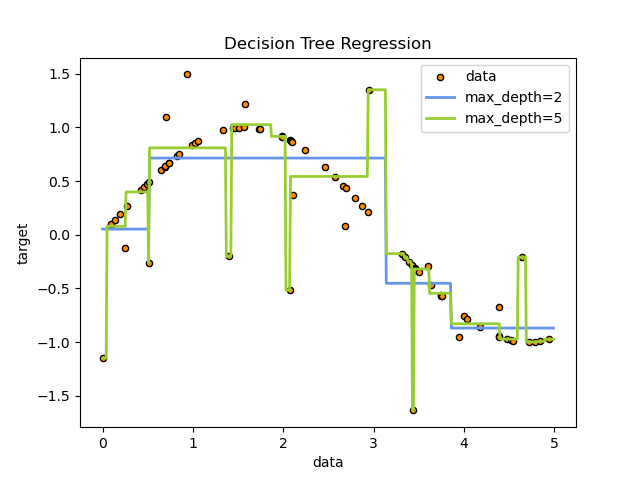
\includegraphics[width=0.5\textwidth]{images/regression_tree.png}
      \caption{Example for decision tree regression model \parencite{110Decis87:online} }
      \label{fig:regtree}
  \end{figure}
\\\\
To avoid the overfitting issue, the model RandomForestRegressor \parencite{sklearne87:online}, is trained which works on the same idea as described for the Random Forest Classification. 

\subsection{Gradient boosting regression}
Combining the idea behind Decision Tree Regression and Gradient Boosting Classification, the Gradient Boosting Regression model can be built. The major difference Gradient Boosting Classification is the fact that the underlying trees being built are regression in nature. 

\section{Pattern recognition}\label{patternreg}
As described in the blog \parencite{Frequent45:online}, pattern recognition is a set of algorithms that identify repetitive patterns in data. The pattern recognition algorithms described in this thesis differ from the classification and regression models in a major aspect. Instead of predicting target features on an unseen dataset, they bring insights into the underlying dataset, by highlighting patterns. This is very useful for the use-case of this thesis, due to the explainable nature.
\\\\
Before the algorithms described in this section are used, it is to be highlighted that a different dataset is used and additional preprocessing steps are executed on top of the ones described in chapter \ref{chapter:preprocessing}. Since the algorithms deal with discrete data with binary features, the dataset needs to be converted into such data. To ease these steps, the input parameters during benchmarking are limited to a defined set of possible values, instead of taking a random value in a given range. Additionally, less features are varied during the benchmarking, to avoid bloating the dimensionality of the data. To achieve the binary features, after dropping static features, \textbf{one-hot encoding} of all features is implemented. The exception to this is the feature \textit{time}, which before being one-hot encoded is split into three sections, similarly to the technique used for the classification models. The choice of three buckets instead of 10 used in classification stems from the limited variations of the input. The goal for these algorithms, in the context of this thesis, is to be able to identify which page size of leaf nodes performs faster for which B+ tree optimizations. 

\subsection{Apriori}
The Apriori algorithm, introduced by Agrawal et al. in \parencite{agrawal1994fast}, is used to identify frequent itemsets. These itemsets are later used in mining for association rules. The algorithm considers only one metric, the \textbf{support} which is defined as the fraction of the amount an itemset occurs in a dataset. After defining a support threshold, the algorithm returns the itemsets with a higher support. 
\\\\
The following example from the \textit{mlxtend} library \parencite{Apriorim11:online} outlines the algorithm. The transactions from figure \ref{fig:apriori1} yield for a minimum threshold of $60\%$ the frequent itemsets in figure \ref{fig:apriori2}.

\begin{figure}[H]
      \centering
      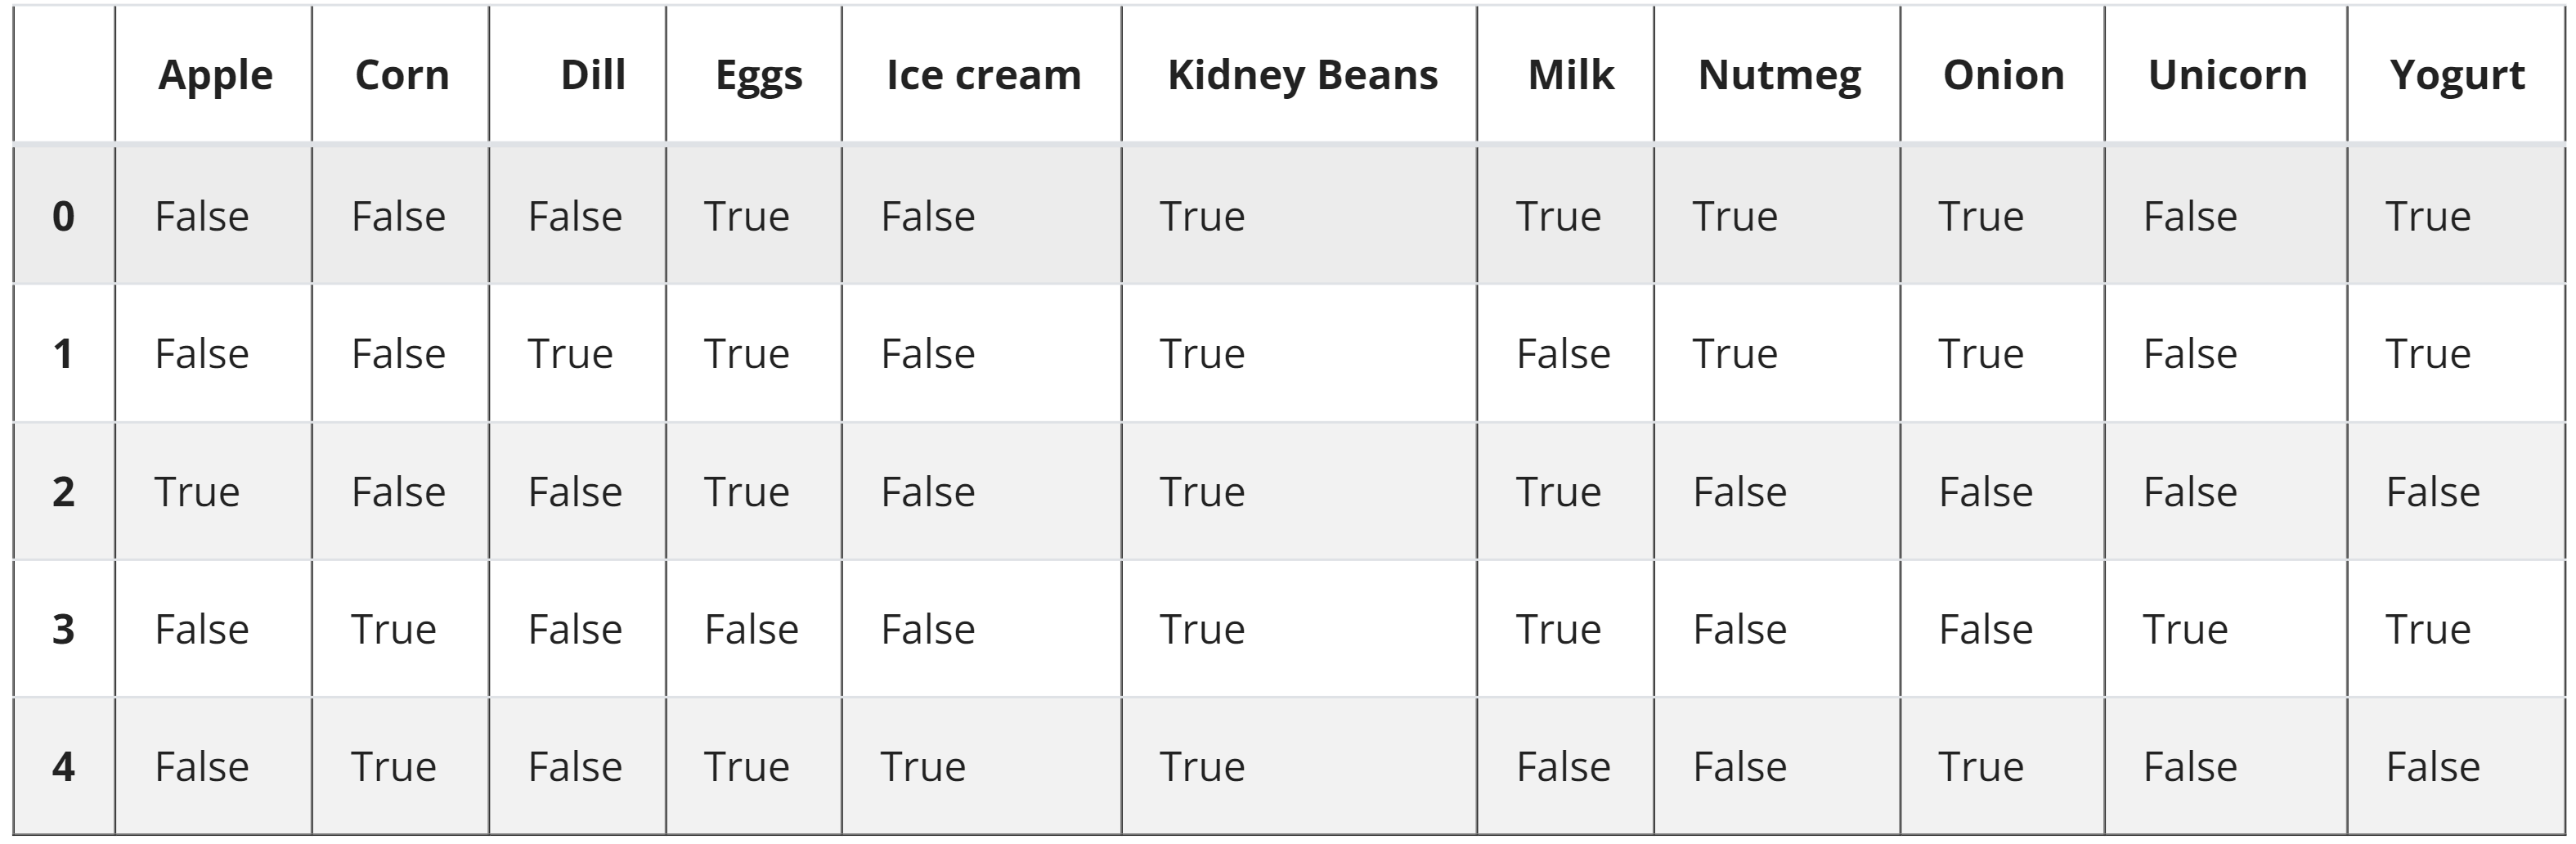
\includegraphics[width=0.5\textwidth]{images/apriori1.png}
      \caption{Apriori input example \parencite{Apriorim11:online} }
      \label{fig:apriori1}
  \end{figure}

\begin{figure}[H]
      \centering
      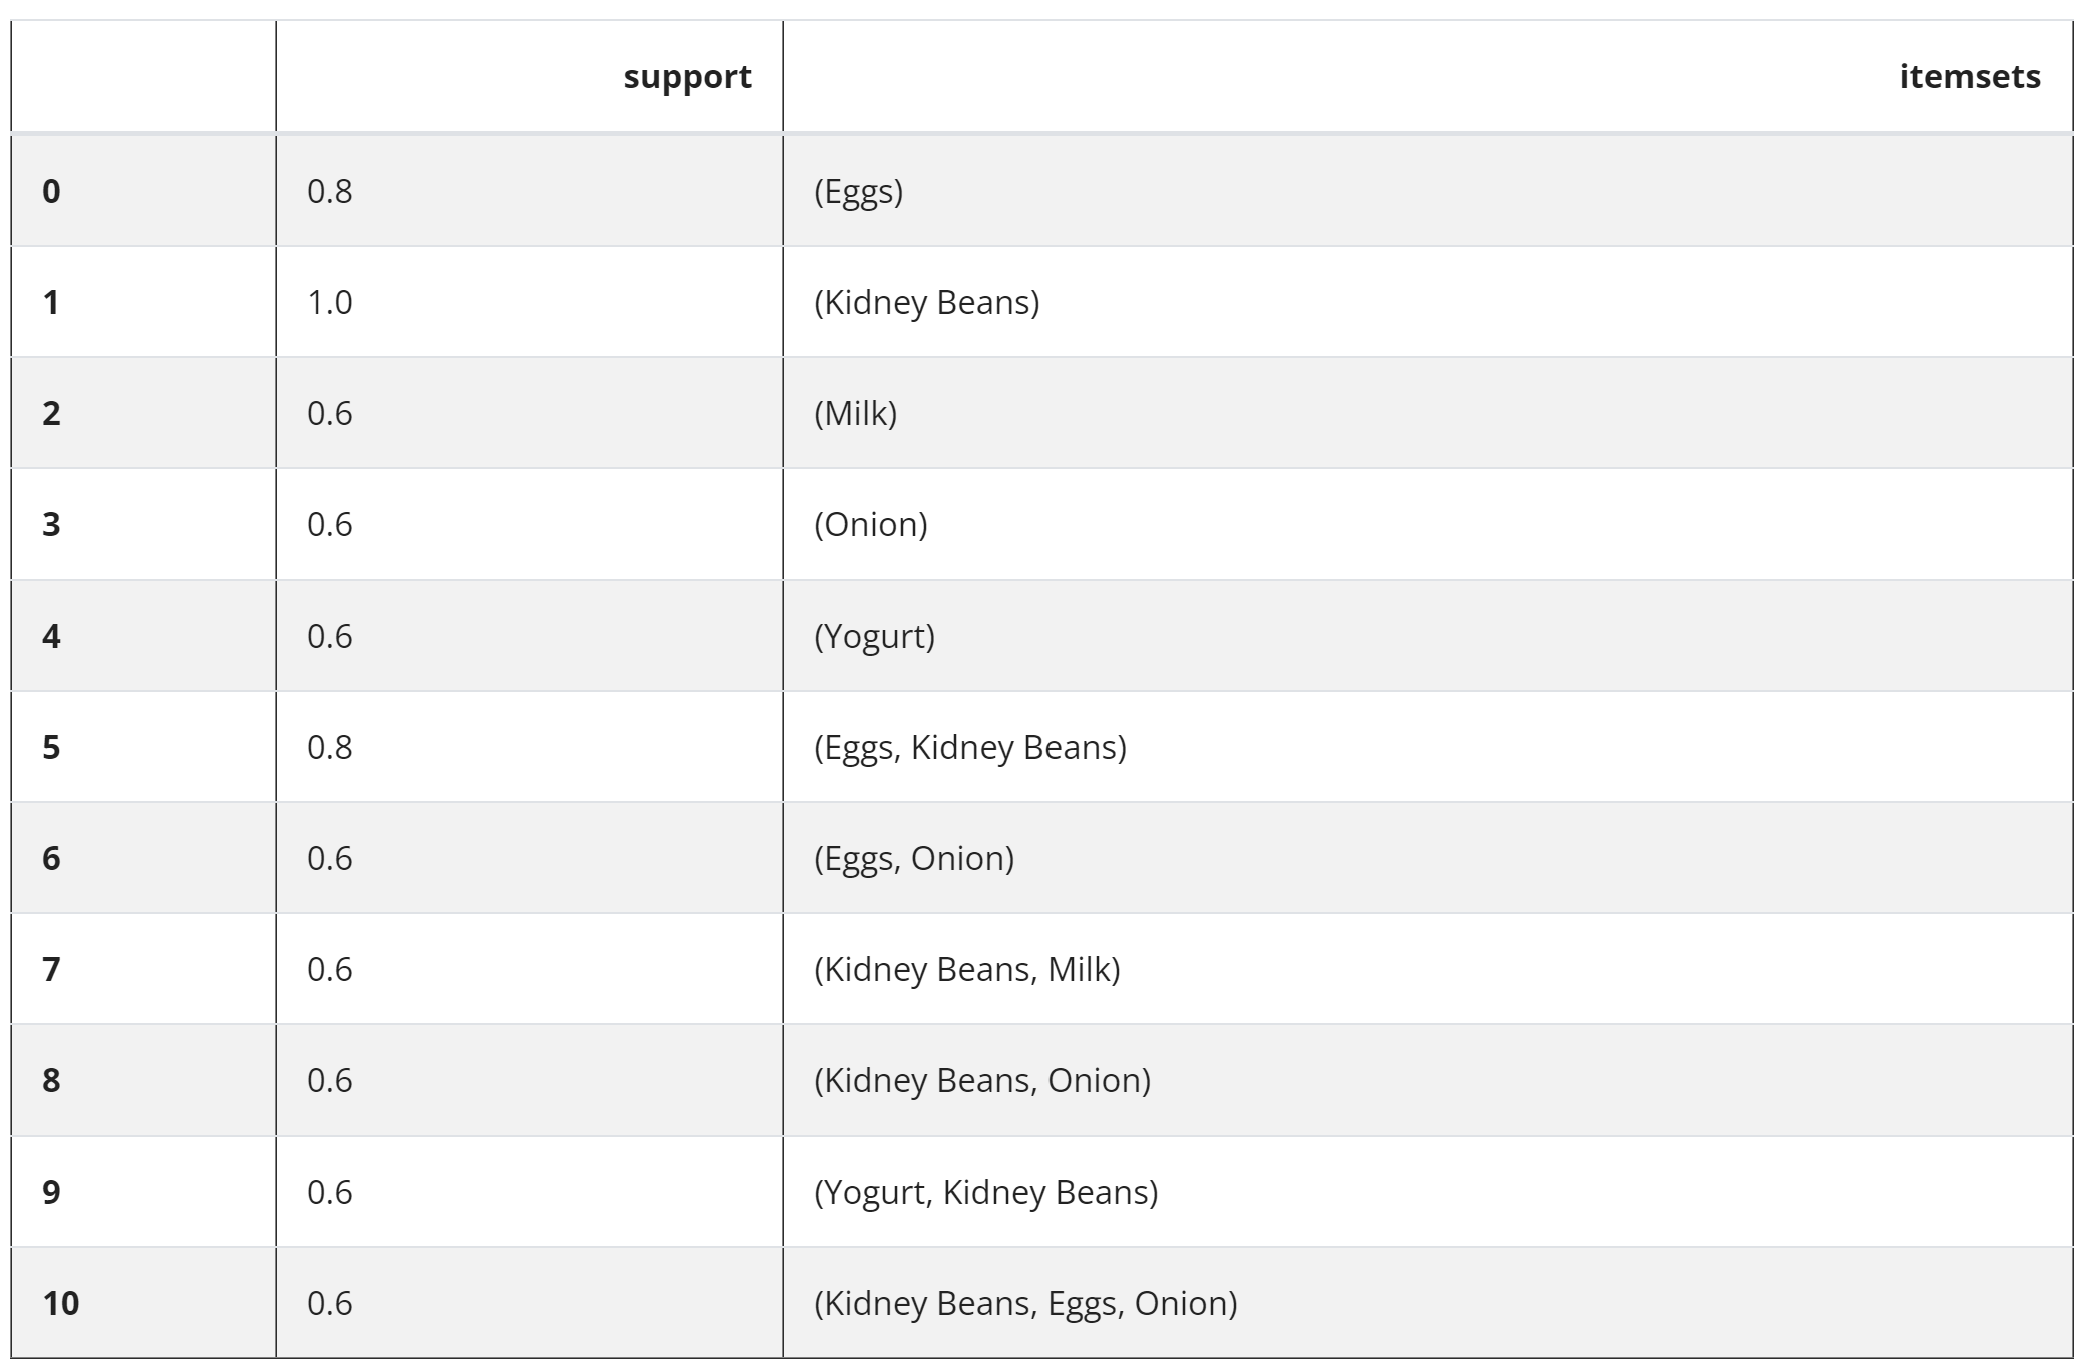
\includegraphics[width=0.5\textwidth]{images/apriori2.png}
      \caption{Apriori output example with $60\%$ support threshold \parencite{Apriorim11:online}}
      \label{fig:apriori2}
  \end{figure}

\subsection{Association rules}
The \textit{mlxtend} library describes association rules in its documentation \parencite{Associat99:online}, as rules in the form of $X \rightarrow Y$ with X and Y being disjoint itemsets. The rules imply the likely existence of $Y$ given that $X$ occurs.
\\\\
The implementation, from the \textit{mlxtend} library \parencite{Associat99:online} used in this thesis, takes the frequent itemsets created by the Apriori algorithm and generates rules based on those. It also allows limiting the output, by allowing to set a threshold for a metric. The implementation calculates various metrics for the rules, such as the ones used in this thesis support, confidence and lift.
\\\\
For $A \rightarrow C$, and A meaning antecedent itemset and C meaning consequent itemset the metrics used are defined by \textit{mlxtend} \parencite{Associat99:online} as follows: 
\begin{itemize}
    \item \textbf{Support:} Equal to the support of the union of the itemsets, described in Apriori algorithm.\\
    \begin{equation}
    \text{support}(A\rightarrow C) = \text{support}(A \cup C), \;\;\; \text{range: } [0, 1]
    \end{equation}
    
    \item \textbf{Confidence:} The conditional probability of finding the consequent item in a transaction given that the transaction contains the antecedent itemset.\\
    \begin{equation}
    \text{confidence}(A\rightarrow C) = \frac{\text{support}(A\rightarrow C)}{\text{support}(A)}, \;\;\; \text{range: } [0, 1]
    \end{equation}
    
    \item \textbf{Lift:} The ratio of the observed support to that expected if the items were statistically independent. It indicates the strength of a rule over random chance. Statistically independent itemsets would have the lift equal to 1. \\
    \begin{equation}
    \text{lift}(A\rightarrow C) = \frac{\text{confidence}(A\rightarrow C)}{\text{support}(C)}, \;\;\; \text{range: } [0, \infty]
    \end{equation}
\end{itemize}

\subsection{Optimal page size of leaf nodes}
To identify the most optimal size of leaf nodes, heatmaps can be generated, which visualize the features \textit{payload\_size} and \textit{data\_size} together with the best performing page size of leaf nodes. For this, two approaches are taken. One of the approaches is taking the dataset created for pattern recognition and training regression models on it. Then for each combination of the features \textit{payload\_size}, \textit{data\_size} and \textit{const\_pageSizeLeaf} the best performing page size is shown in the respective section. The other approach is skipping the regression model step and taking the empirical mean performance instead to identify the optimal page size. \\\\
The results of these approaches are outlined in chapter \ref{chapter:findings}. 